%%%%%%%%%%%%%%%%%%%%%%%%%%%%%%%%%%%%%%%%%%%%%%%%%%%%%%%%%%%%%%%%%%%%%%
%
%
%
%%%%%%%%%%%%%%%%%%%%%%%%%%%%%%%%%%%%%%%%%%%%%%%%%%%%%%%%%%%%%%%%%%%%%%
%\documentclass[12pt,preprint]{aastex}
\documentclass[iop, twocolumn, tighten]{emulateapj}
\usepackage{amsmath}
\usepackage{color}
\definecolor{grey}{rgb}{0.5,0.5,0.5}
\definecolor{red}{rgb}{0.8,0.0,0.0}
\usepackage{listings}

\newcommand{\Vb}{{\boldsymbol V}}
\newcommand{\vb}{{\boldsymbol v}}
%\newcommand{\vtb}{{\boldsymbol \tilde{v}}}
\newcommand{\vtb}{{\tilde{ \boldsymbol  v}}}
\newcommand{\Tf}{{\mathcal{T}}}
\newcommand{\Xt}{{\tilde{X}}}
\newcommand{\Yt}{{\tilde{Y}}}
\newcommand{\Zt}{{\tilde{Z}}}
\newcommand{\Vp}{V_p}
\newcommand{\Vsys}{V_\mathrm{sys}}


%%%%%%%%%%%%%%%%%%%%%%%%%%%%%%%%%%%%%%%%%%%%%%%%%%%%%%%%%%%%%%%%%%%
\slugcomment{}
\shortauthors{}
\shorttitle{}
\bibliographystyle{apj}

%%%%%%%%%%%%%%%%%%%%%%%%%%%%%%%%%%%%%%%%%%%%%%%%%%%%%%%%%%%%%%%%%%%%%%
\begin{document}
%%%%%%%%%%%%%%%%%%%%%%%%%%%%%%%%%%%%%%%%%%%%%%%%%%%%%%%%%%%%%%%%%%%%%%
\title{ChopStacks}
%%%%%%%%%%%%%%%%%%%%%%%%%%%%%%%%%%%%%%%%%%%%%%%%%%%%%%%%%%%%%%%%%%%%%%

%%%%%%%%%%%%%%%%%%%%%%%%%%%%%%%%%%%%%%%%%%%%%%%%%%%%%%%%%%%%%%%%%%%%%%
\author{Hajime Kawahara\altaffilmark{1,2}}
\email{kawahara@eps.s.u-tokyo.ac.jp}
\altaffiltext{1}{Department of Earth and Planetary Science, 
The University of Tokyo, Tokyo 113-0033, Japan}
\altaffiltext{2}{Research Center for the Early Universe, 
School of Science, The University of Tokyo, Tokyo 113-0033, Japan}

%%%%%%%%%%%%%%%%%%%%%%%%%%%%%%%%%%%%%%%%%%%%%%%%%%%%%%%%%%%%%%%%%%%%%%
\begin{abstract}
ChopStacks is a python code collection for resampling data and stacking them under the flux preservation.
\end{abstract}
\keywords{}
%%%%%%%%%%%%%%%%%%%%%%%%%%%%%%%%%%%%%%%%%%%%%%%%%%%%%%%%%%%%%%%%%%%%%%

\section{Introduction}
We sometimes need to re-sample 1D discrete data (i.e. spectra, light curves, and so on). Of course, the interpolation is one of the major solutions to this problem. However, we sometimes need the flux preservation simultaneously, for instance, when we stack the data.My Python small package, Chopstacks, provides the functions, 

\begin{itemize}
\item re-sampling 1D data and preserving flux with an arbitrary array, 
\item stacking 1D data with preserving flux,
\item converting the 1D data into the log 1D data with preserving flux.
\end{itemize}

This document describes the background mathematics of Chopstacks. If you want to know how to use, read jupyter notebooks in ipynb directory.

\section{Algorithm}

I consider the situation that the stacked spectrum (we use the term of "spectrum" as an example of 1D data) $\hat{f}(x)$ consists of the sum of $M$-spectra as 
\begin{eqnarray}
  \hat{f} (x) = \sum_{m=0}^{M-1} f^{(m)} (x)
\end{eqnarray}
I assume that the stacked spectrum and each spectrum have the unit of [$q/X$], where $q$ is the unit of preserved quantity $Q(x)$ and $X$ is the unit of $x$.

%%%%%%%%%%%%%%%%%%%%%%%%%%%%%%%%%%%%%%%%%%%%%%%%%%%%%%%%%%%%%%%%%%%%%
%\begin{figure}[htb]
%  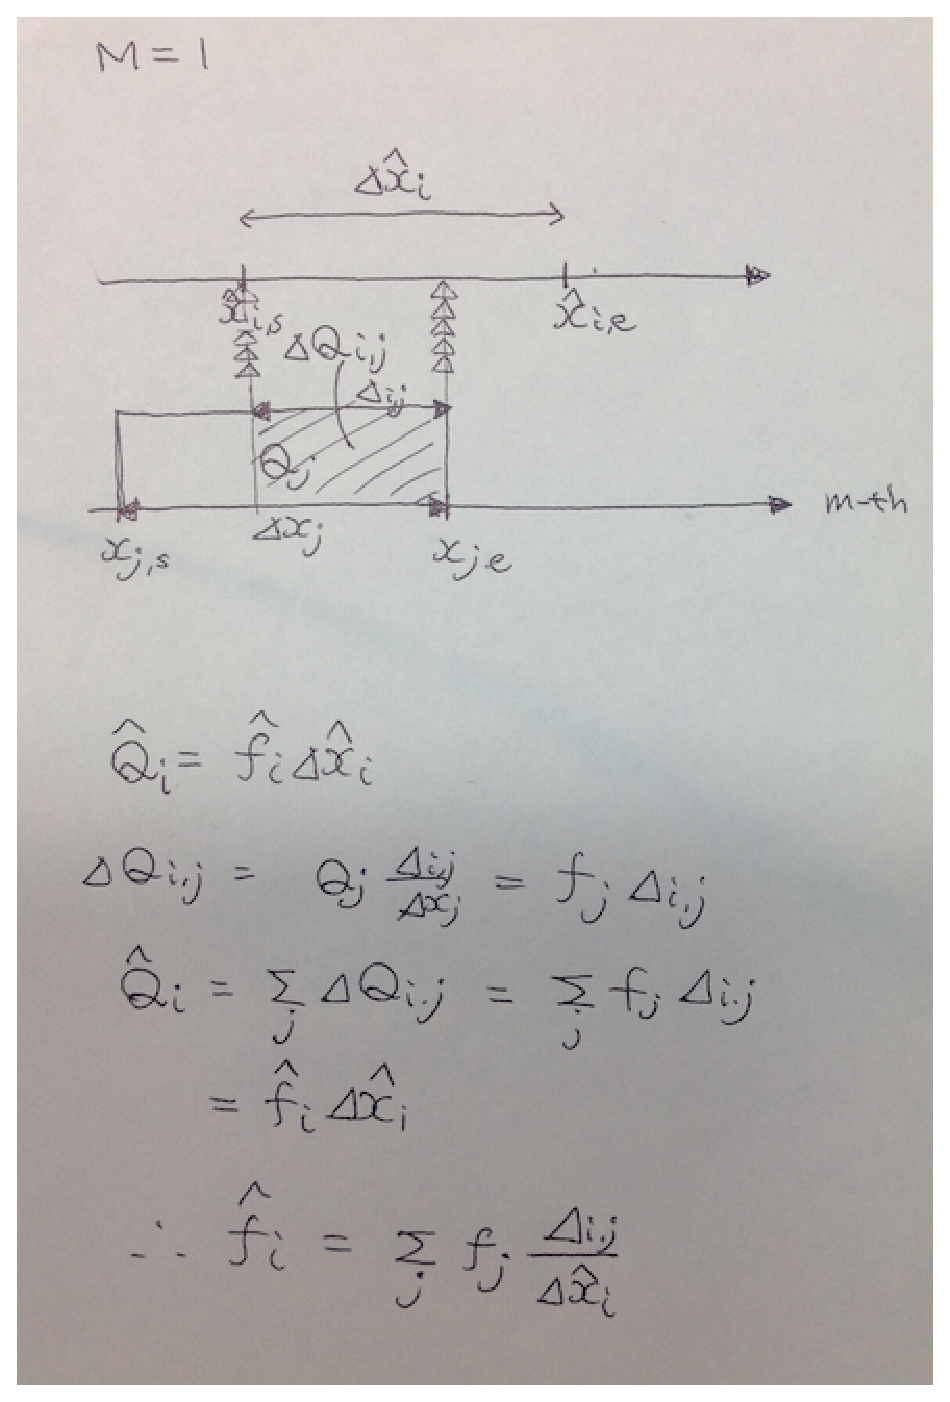
\includegraphics[width=1.0\linewidth]{FIG1.eps}
%\caption{\label{fig:1}}
%\end{figure}
%%%%%%%%%%%%%%%%%%%%%%%%%%%%%%%%%%%%%%%%%%%%%%%%%%%%%%%%%%%%%%%%%%%%%

The stacked spectrum $\hat{f}$ is discretized to the master bin as
\begin{eqnarray}
  \hat{f}_i &\equiv& \hat{f} (\hat{x}_i)  \\
  \hat{x}_i  &:& i = 0,1..,N-1. \\
  f^{(m)}_j &\equiv& f^{(m)} (x_j)  \\
  x_j  &:& j = 0,1..,N-1.
\end{eqnarray}
The width of each bin $\hat{x}_i$ is defined by $\hat{x}_{i,s}$ and $\hat{x}_{i,e}$ as 
\begin{eqnarray}
\Delta \hat{x}_i \equiv \hat{x}_{i,e} - \hat{x}_{i,s}. 
\end{eqnarray}
The quantity in the $i$-th bin is written as
\begin{eqnarray}
\label{eq:tot}
\hat{Q}_i = \hat{f}_i \Delta \hat{x}_i
\end{eqnarray}
and 
\begin{eqnarray}
Q^{(m)}_j = f^{(m)}_j \Delta x^{(m)}_j. 
\end{eqnarray}

The problem is how to distribute the quantity in $\hat{f}_i$ from $f^{(m)}_j$. I denote the overlaped region between $\hat{x}_i$ and $x^{(m)}_j$ by $\Delta^{(m)}_{i,j}$. Then the contribution of the $j$-th bin of the $m$-th spectra to $\hat{Q}_i$  is 
\begin{eqnarray}
\Delta Q^{(m)}_{i;j} &=& Q^{(m)}_j \frac{\Delta^{(m)}_{i,j}}{\Delta x^{(m)}_j} \\
                   &=& f^{(m)}_j \Delta^{(m)}_{i,j}
\end{eqnarray}

Hence, the quantity in the i-th stacked bin is 
\begin{eqnarray}
\hat{Q}_i &=& \sum_{m=0}^{M-1} \sum_j \Delta Q^{(m)}_{i;j} \\
&=& \sum_{m=0}^{M-1} \sum_j f^{(m)}_j  \Delta^{(m)}_{i,j}. 
\end{eqnarray}
Using equation (\ref{eq:tot}), I obtain
\begin{eqnarray}
\hat{f}_i = \sum_{m=0}^{M-1} \sum_{j=0}^{N-1} f^{(m)}_j \frac{\Delta^{(m)}_{i,j}}{\Delta \hat{x}_i}.\nonumber \\
\end{eqnarray}
Though this eqution has $M \times N$ terms, however, most of $\Delta^{(m)}_{i,j}$ is zero. Hence, it is faster if I can find the overlap $(i,j)$ which satisfies $\Delta^{(m)}_{i,j} \ne 0$ for each spectrum.
\begin{eqnarray}
\hat{f}_i = \sum_{m=0}^{M-1} \sum_{j \in \mathrm{overlap}} f^{(m)}_j \frac{\Delta^{(m)}_{i,j}}{\Delta \hat{x}_i}. 
\end{eqnarray}

\subsection{implementation}

{\bf chopstacks.py} is the central program of this algorithm. The main subroutine to redistribute the value is {\bf cutput} in {\bf chopstacks.py}. The illustrative explanation of this routine is shown in Figure \ref{fig:ssp}. 
The input arrays of {\bf cutput} are 
\begin{itemize}
\item xw: walls of the original bins [X], i.e. (N)-array.   
\item f: input value [q/X], i.e. (N-1)-array.   
\item hxw: walls of the resampled bins [X], i.e. (N)-array.   
\item hf: stacking array [q/X], i.e. (N-1)-array, 
\end{itemize}
and the output is 
\begin{itemize}
\item hf: the input hf + resampled and stacked data.
\end{itemize}
Because 1D data often use the representative values of [X] (usually, the central value of the bin), you need to set $N$-walls between the $(N-1)$-representative values of [X].   
If you want to set the walls to be the center of the neighboring representative values, use {\bf buildwall} in chopstacks.py. The edge option specifies the deal of the edge values. If you specify hf=None, then chopstacks.py assumes the initial hf to be a zero array. So, if you just want to divide the 1D data, use hf=None.  

%%%%%%%%%%%%%%%%%%%%%%%%%%%%%%%%%%%%%%%%%%%%%%%%%%%%%%%%%%%%%%%%%%%%%
\begin{figure}[]
  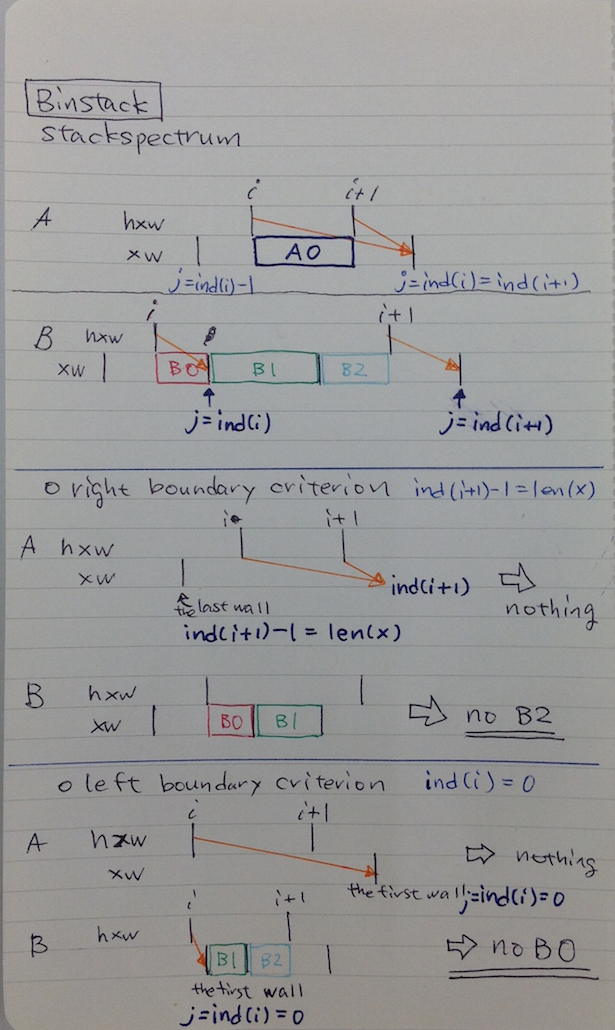
\includegraphics[bb=0 0 615 1030,width=\linewidth]{stackspectrum.png}
\caption{Schematic explanation of {\bf cutput}. The code is shown in appendix. \label{fig:ssp}}
\end{figure}
%%%%%%%%%%%%%%%%%%%%%%%%%%%%%%%%%%%%%%%%%%%%%%%%%%%%%%%%%%%%%%%%%%%%%

\newpage

\section{Applications}
 Use the spectra with the unit of [$q/X$]. The preservation of $q$ can be checked using {\bf check\_preservation}.

\subsection{Log Bin Convertor}

{\bf analogbin.py} performs the resampling of $f$ [$q/X$] into the logscale of $x$ ($l \equiv \log x$) with a resolution power $R$. The relation between $\delta \log x$ and R is provided by
\begin{eqnarray}
\Delta l \equiv \delta \log x = \frac{\Delta x}{x} = \frac{1}{R}.
\end{eqnarray}
Then the number of the rebinned data is given by 
\begin{eqnarray}
\hat{N} = \frac{\log \hat{x}_N  - \log \hat{x}_0}{\Delta l} = R (\log \hat{x}_N  - \log \hat{x}_0).
\end{eqnarray}

The {\bf opt} option specifies the output form. opt=0 will provide
\begin{itemize}
\item $\hat{x}$, walls of $\hat{x}$, $\hat{f}$.
\end{itemize}
opt=1 provides
\begin{itemize}
\item $\log \hat{x}$, walls of $\log \hat{x}$, $\hat{x} \hat{f}$.
\end{itemize}
The latter output is based on the preservation law
\begin{eqnarray}
f d x &=& f \left| \frac{\partial x}{\partial (\log x)}\right| d (\log) x \nonumber \\
&=&   x f d (\log x).
\end{eqnarray}
Subroutine {\bf check\_preservation} can check the degree of preservation of $[q]$. 

%%%%%%%%%%%%%%%%%%%%%%%%%%%%%%%%%%%%%%%%%%%%%%%%%%%%%%%%%%%%%%%%%%%%%
\begin{figure*}[!htb]
  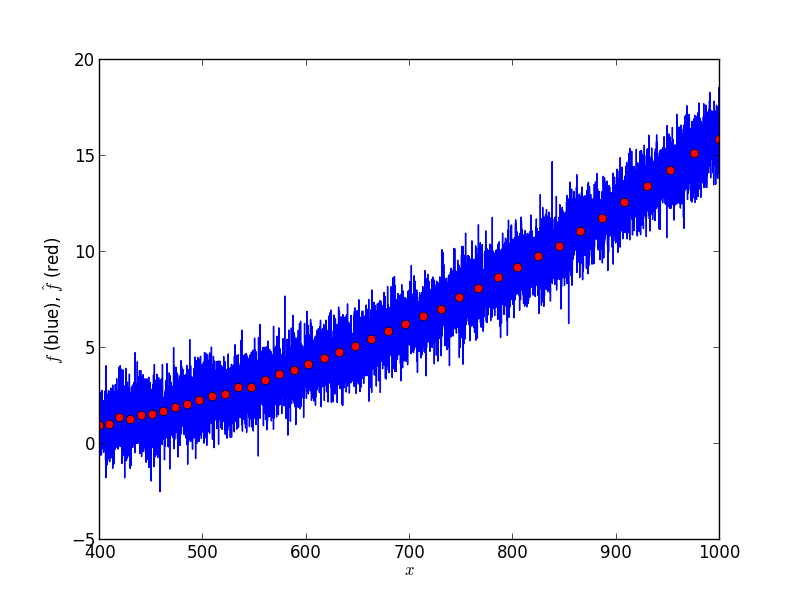
\includegraphics[bb=0 0 576 432,width=0.49\linewidth]{demo1.png}
  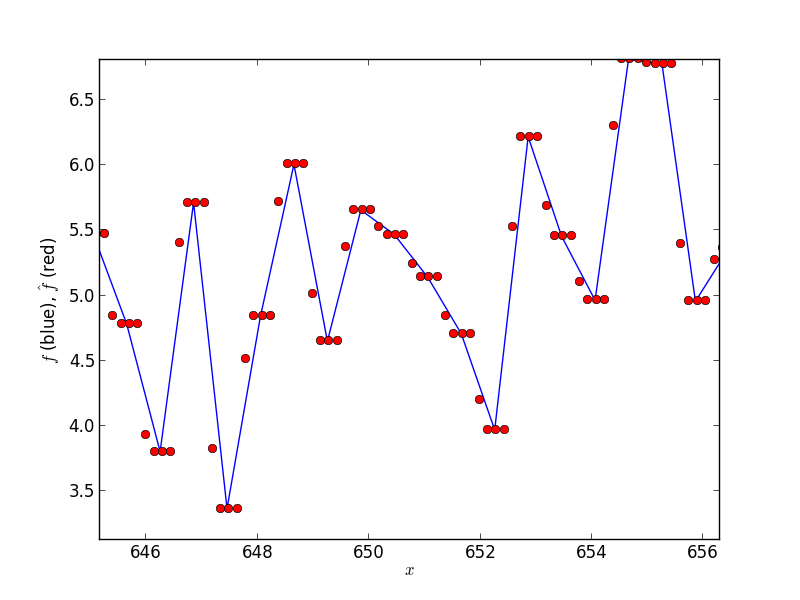
\includegraphics[bb=0 0 576 432,width=0.49\linewidth]{demo2.png}
\caption{Demonstrations of the log binning. The blue line is original data and the red one is the binned data. The right panel shows the oversampling case. \label{fig:2}}
\end{figure*}
%%%%%%%%%%%%%%%%%%%%%%%%%%%%%%%%%%%%%%%%%%%%%%%%%%%%%%%%%%%%%%%%%%%%%

\newpage
\appendix

\small
\begin{verbatim}
def cutput(xw,f,hxw,hf=None,silent=None):
    #see note 14.8.12 and 14.9.02
    if hf is None:
        if silent is None:
            print "Reset master data (hf) to zero."
        hf=np.zeros(len(hx))

    ind=np.digitize(hxw,xw)
    for i in range(0,len(hxw)-1):

        if ind[i]<len(xw) and ind[i+1]-1 < len(xw)+1 and ind[i]>0:  #cx1,cx2,cx3
            if ind[i]==ind[i+1]:
                hf[i]=hf[i]+f[ind[i]-1] #A0
            else: 
                hf[i]=hf[i]+f[ind[i]-1]*(xw[ind[i]]-hxw[i])/(hxw[i+1]-hxw[i]) #B0
                for k in range(ind[i]+1, ind[i+1]):
                    hf[i]=hf[i]+f[k-1]*(xw[k]-xw[k-1])/(hxw[i+1]-hxw[i]) #B1    
                hf[i]=hf[i]+f[ind[i+1]-1]*(hxw[i+1]-xw[ind[i+1]-1])/(hxw[i+1]-hxw[i]) #B2

        elif ind[i+1]-1 == len(xw)+1:  #right boundary criterion
            if ind[i]<ind[i+1]:
                hf[i]=hf[i]+f[ind[i]-1]*(xw[ind[i]]-hxw[i])/(hxw[i+1]-hxw[i]) #B0            
                for k in range(ind[i]+1, ind[i+1]):
                    hf[i]=hf[i]+f[k-1]*(xw[k]-xw[k-1])/(hxw[i+1]-hxw[i]) #B1    
                                        
        elif ind[i]==0 and ind[i+1]>0: #left boundary condition
                for k in range(ind[i]+1, ind[i+1]):
                    hf[i]=hf[i]+f[k-1]*(xw[k]-xw[k-1])/(hxw[i+1]-hxw[i]) #B1    
                hf[i]=hf[i]+f[ind[i+1]-1]*(hxw[i+1]-xw[ind[i+1]-1])/(hxw[i+1]-hxw[i]) #B2
 
    return hf
\end{verbatim}

\end{document}
